\chapter{Scenario Implementation and Results}
% Introduction
This chapter presents results of two scenarios using the proposed navigation filter and its underlying components discussed in previous chapters. Both scenarios use a similar trajectory and will be discussed thoroughly to avoid confusion. First, the chapter starts with a discussion of the first scenario and the five separate cases run in Monte-Carlo for scenario one. Following a description of scenario one, results from specific cases will be presented, highlighting the strong and weak points of the proposed navigation filter. The results from the remaining cases not presented in this chapter can be found in the appendix of this work. Once the analysis of scenario one has concluded, a description of scenario two is presented, followed by Monte-Carlo statistical analyses. The performance of the proposed navigation filter will be determined based on 100-run Monte-Carlo simulations each scenario and and each case. As a visual comparison, a loosely-coupled IMU is added for the same scenarios.

\section{\textbf{Simulated Trajectory}}
As stated previously, both scenarios one and two will be flying a similar trajectory. This trajectory meets the observability criteria discussed in Chapter 5, featuring continuous banking of the aircraft with a steady climb to provide excitation to the angular states for better estimates of the orientation during simulations. Figure~\ref{fig:trajectory} presents the \textit{S}-like trajectory and Table~\ref{tbl:trajectory} presents the initial conditions of the simulated Diamond DA-40.

\begin{figure}[!ht]
    \centering
    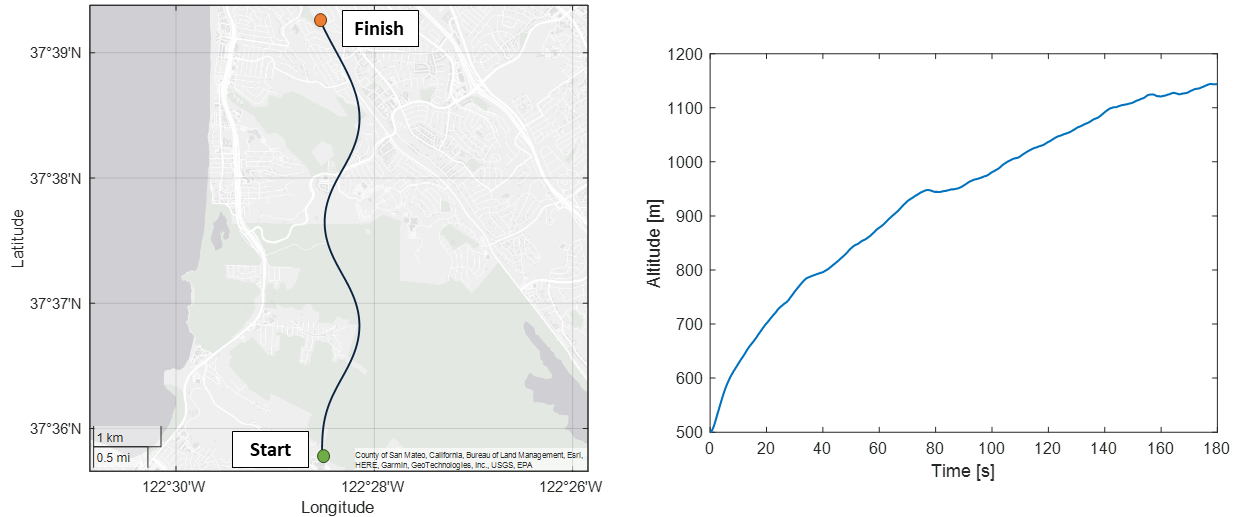
\includegraphics[width=\linewidth]{Figures/trajectoryfigure.png}
    \caption{Simulated trajectory for both presented scenarios with accompanying altitude flightpath. }\label{fig:trajectory}
\end{figure}

\begin{table}[!ht]
    \caption{Initial conditions for simulated trajectory from Figure~\ref{fig:trajectory}.}\label{tbl:trajectory}
    \centering
    \begin{tabular}{lcc}
        \toprule
        \textbf{Condition}       & \textbf{Value}                                      & \textbf{Units}                     \\
        \midrule
        Date                     & June 15, 2022                                       & \textit{DateTime} Object           \\
        Duration                 & 180                                                 & \(s\)                              \\
        Monte-Carlo Runs         & 100                                                 & {--}                               \\
        Frequency                & 200                                                 & Hz                                 \\
        Trajectory               & \textit{SCurveFlightPath.mat}                       & See Chapter 5                      \\
        Velocity Disturbance     & \(\left[300, \; 300, \; 0\right]\)                  & \(m/s\)                            \\
        Angular Rate Disturbance & \(\left[10^{-12}, \; 10^{-12}, \; 10^{-12}\right]\) & \(rad/s\)                          \\
        Position Disturbance     & \(\left[0, \; 0, \; 10\right]\)                     & \(m\)                              \\
        Clock Type               & OCXO                                                & {--}                               \\
        Initial Velocity         & \(\left[75, \; 0, \; 0\right]\)                     & \(m/s\)                            \\
        Initial Angular Rate     & \(\left[0, \; 0, \; 0\right]\)                      & \(rad/s\)                          \\
        Initial Position         & \(\left[0.65617, \; -2.1376, \; 500\right]\)        & \(\left[rad, \; rad, \; m\right]\) \\
        Initial Attitude         & \(\left[0, \; 0, \; 0\right]\)                      & \(rad\)                            \\
        Initial Clock Terms      & \(\left[0, \; 0\right]\)                            & \(\left[m, \; m/s\right]\)         \\
        Channel \(C/N_0\)        & \(45\)                                              & db-Hz                              \\

        \bottomrule
    \end{tabular}
\end{table}

From Table~\ref{tbl:trajectory}, several parameters are configurable to meet the desired simulation of the user. Date is used to pull the specified Rinex file from~\cite{CDDIS}. This Rinex file is then parsed for its ephemeris and used to propagate the satellites during the simulation. SGP4 propagation~\cite{} is used to propagate the satellites PVT during simulation. Because simulations are not expected to be more than four hours long, this propagation method stays within its error criteria and is okay to use for the purpose of this thesis. Figure~\ref{fig:skyplot} shows the available satellites at the first time step for June 15, 2022 used in this work.

\begin{figure}[!ht]
    \centering
    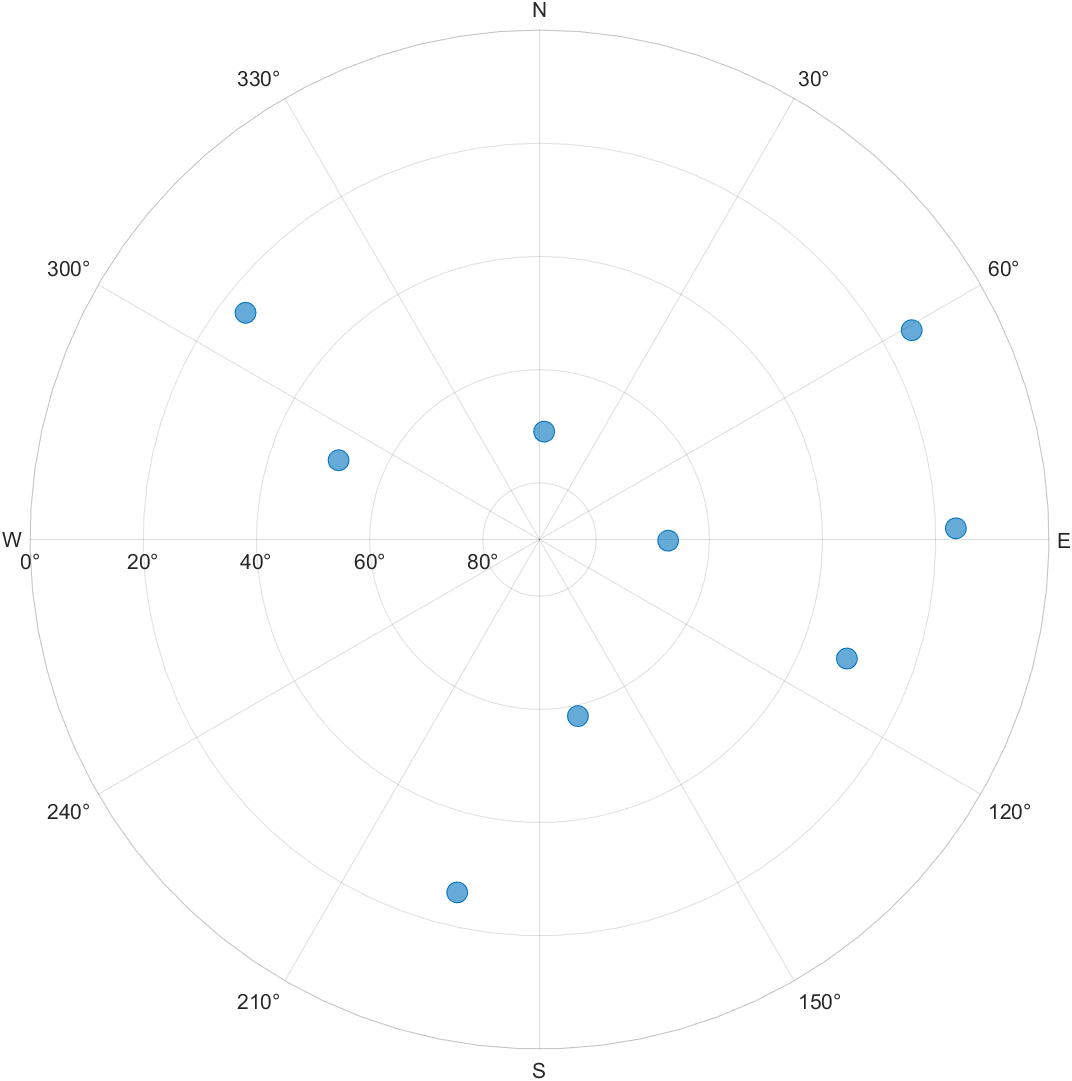
\includegraphics[width=0.4\linewidth]{Figures/Results/skyplot.png}
    \caption{Skyplot of the available satellites during the simulation of both scenarios given the date of broadcast ephemeris.}\label{fig:skyplot}
\end{figure}

Duration and Monte-Carlo Runs specify the length of each simulation in seconds and the number of simulations for each scenario and/or case. For the work presented in thesis, 100 simulation Monte-Carlo runs are used for analyses. This may not seems substantial, but based on~\cite{khaghaniAssessmentVDMbasedAutonomous2018,khaghaniAutonomousVehicleDynamic2016,mwenegohaModelbasedTightlyCoupled2020} and time to completion for each simulation, 100 simulations is enough to show the general trend for statistical purposes.

The trajectory is specified as a -mat file. The creation of the trajectory file is detailed in Chapter 5. As mentioned before, the S-like trajectory is to provided excitation in the angular states for better estimates during simulation. 

As explained in chapter 5, disturbances are modeled onto the trajectory of the aircraft as the FVDM is not perfect. External conditions such as wind and various atmospheric conditions alter the behavior of the Diamond DA-40 slightly. These disturbances are defined as Velocity, Angular Rate, and Position Disturbance in Table~\ref{tbl:trajectory}.

Clock Type is the embedded receiver clock modeled during the simulation. More information on the different types of clocks can be found in Chapter 4. For the purposes of this thesis, both scenarios and all cases will use the OCXO\@.

The initial states of the aircraft are defined by the accompanying variables. Since our trajectory specifies a mostly-north flight path, the north velocity component is specified to be 75 meters per second, while the other components are zero. Also, the pitch of the aircraft is specified as 4 degrees up, this is so the aircraft generates lift at the first couple time steps during the simulations and does not enter a stall. Lastly, the initial position of the aircraft is specified as the first waypoint location, for simplicity. 

The last configurable parameter is the initial Channel \(C/N_0\) of the available satellites. Because each scenario and case analyzed in this thesis starts in benign conditions, the Channel \(C/N_0\) is defined as \(45\) dB-Hz.

\section{\textbf{Scenario 1}}

\subsection{\textbf{Interference Overview}}

\begin{figure}[!ht]
    \centering
    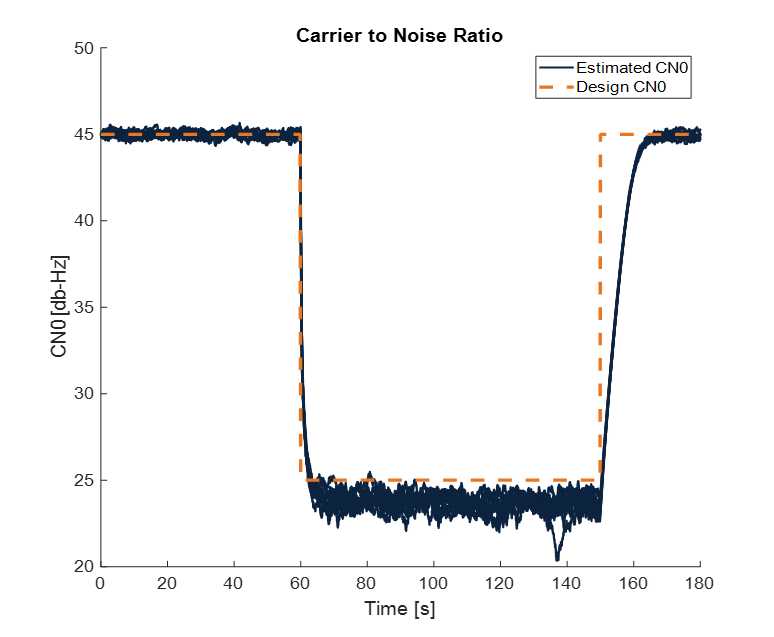
\includegraphics[width=0.75\linewidth]{Figures/Results/CN025.png}
    \caption{Estimated \(C/N_0\) compared with a design \(C/N_0\) that suddenly drops at \(60\) seconds and then dissipates at \(150\) seconds. }\label{fig:CN025}
\end{figure}


\subsection{\textbf{Monte-Carlo Analyses}}
\begin{figure}[!ht]
    \centering
    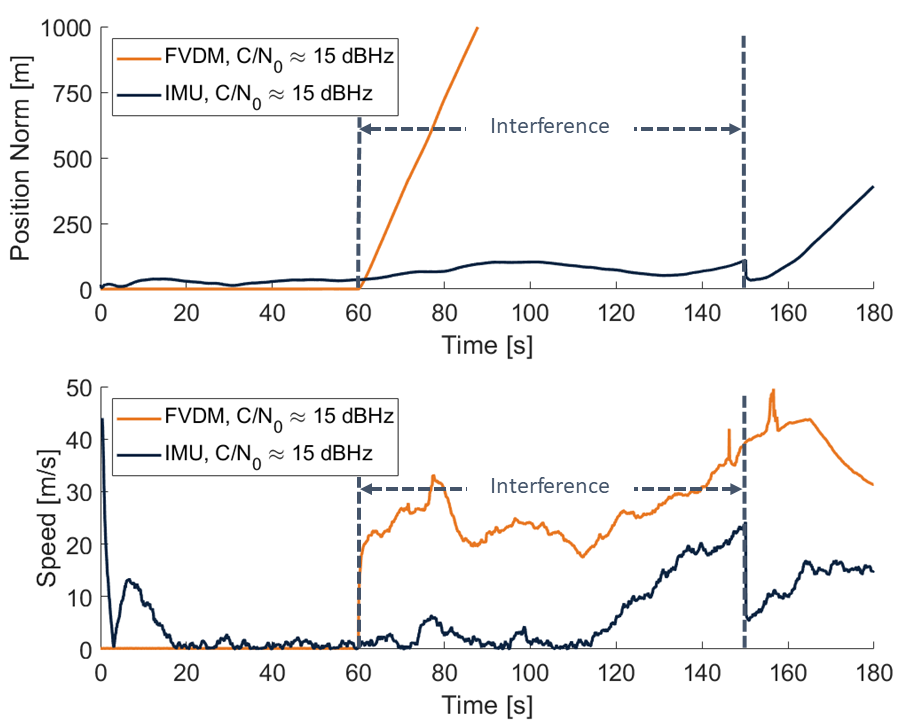
\includegraphics[width=0.75\linewidth]{Figures/Results/trajectoryfigure/Slide14.PNG}
    \caption{Position and speed estimates using the proposed navigation filter when subject to instantaneous interference, bringing the \(C/N_0\) to \(15\) dB-Hz.}\label{fig:PosVel15}
\end{figure}

\begin{figure}[!ht]
    \centering
    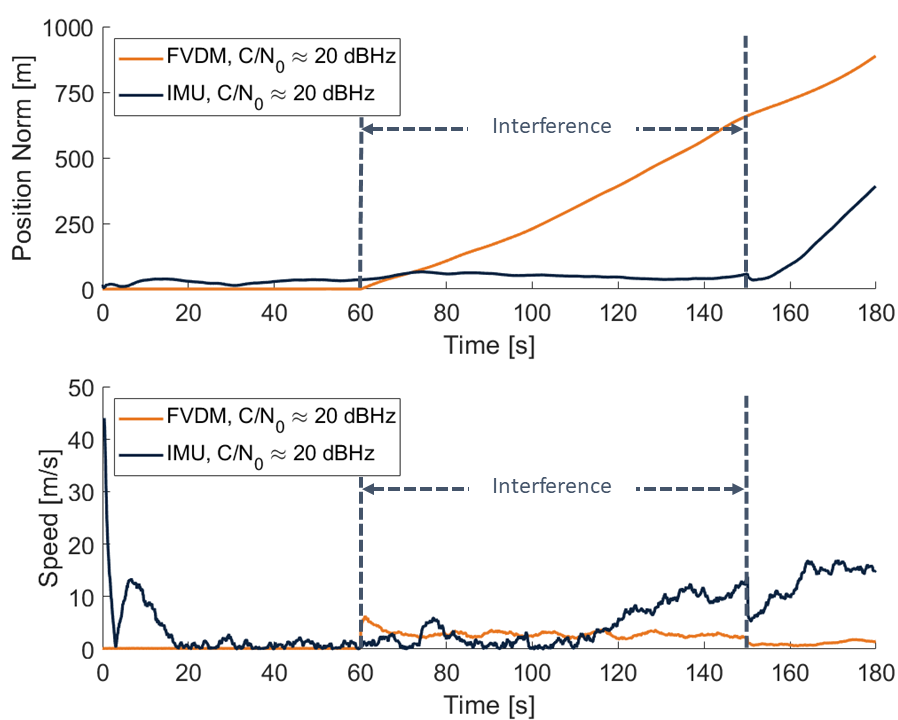
\includegraphics[width=0.75\linewidth]{Figures/Results/trajectoryfigure/Slide15.PNG}
    \caption{Position and speed estimates using the proposed navigation filter when subject to instantaneous interference, bringing the \(C/N_0\) to \(20\) dB-Hz.}\label{fig:PosVel20}
\end{figure}

\begin{figure}[!ht]
    \centering
    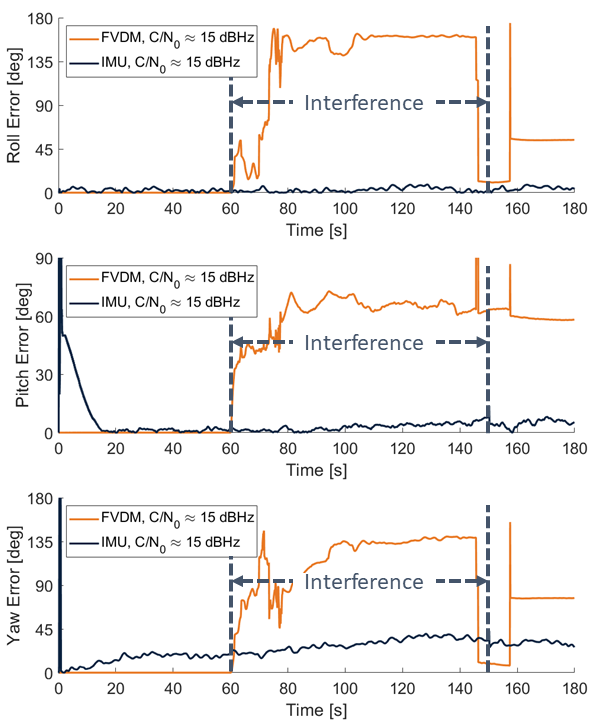
\includegraphics[width=0.75\linewidth]{Figures/Results/trajectoryfigure/Slide2.PNG}
    \caption{Euler attitude estimates using the proposed navigation filter when subject to instantaneous interference, bringing the \(C/N_0\) to \(15\) dB-Hz.}\label{fig:Eul15}
\end{figure}

\begin{figure}[!ht]
    \centering
    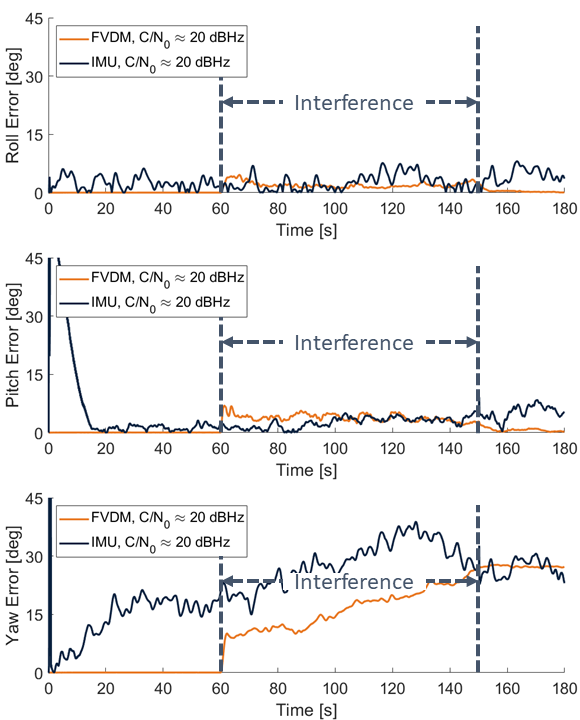
\includegraphics[width=0.75\linewidth]{Figures/Results/trajectoryfigure/Slide3.PNG}
    \caption{Euler attitude estimates using the proposed navigation filter when subject to instantaneous interference, bringing the \(C/N_0\) to \(20\) dB-Hz.}\label{fig:Eul20}
\end{figure}

\begin{figure}[!ht]
    \centering
    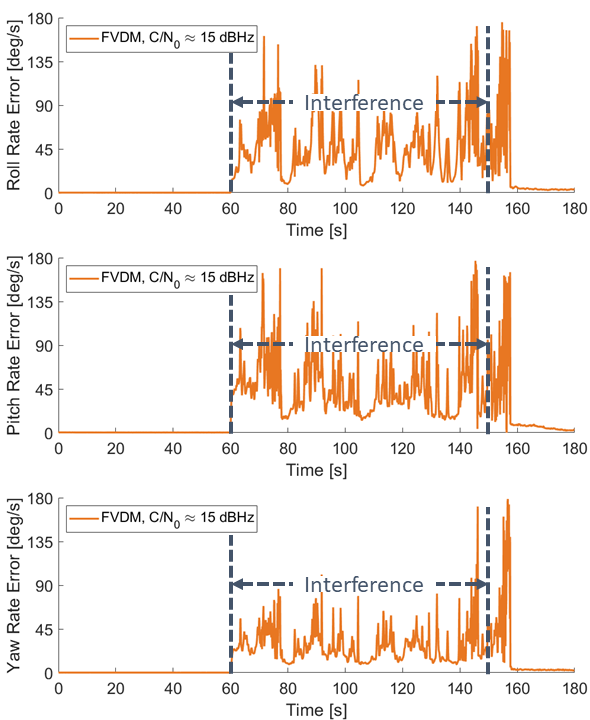
\includegraphics[width=0.75\linewidth]{Figures/Results/trajectoryfigure/Slide8.PNG}
    \caption{Angular rate estimates using the proposed navigation filter when subject to instantaneous interference, bringing the \(C/N_0\) to \(15\) dB-Hz.}\label{fig:Ang15}
\end{figure}

\begin{figure}[!ht]
    \centering
    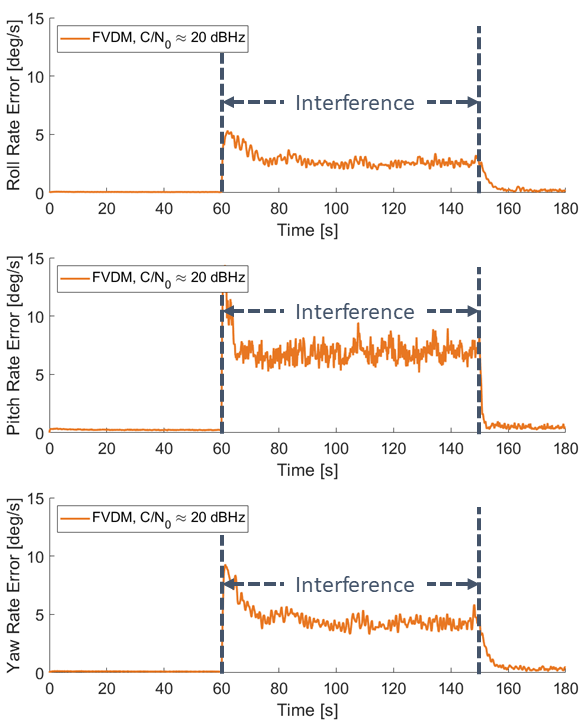
\includegraphics[width=0.75\linewidth]{Figures/Results/trajectoryfigure/Slide9.PNG}
    \caption{Angular rate estimates using the proposed navigation filter when subject to instantaneous interference, bringing the \(C/N_0\) to \(20\) dB-Hz.}\label{fig:Ang20}
\end{figure}

\begin{figure}[!ht]
    \centering
    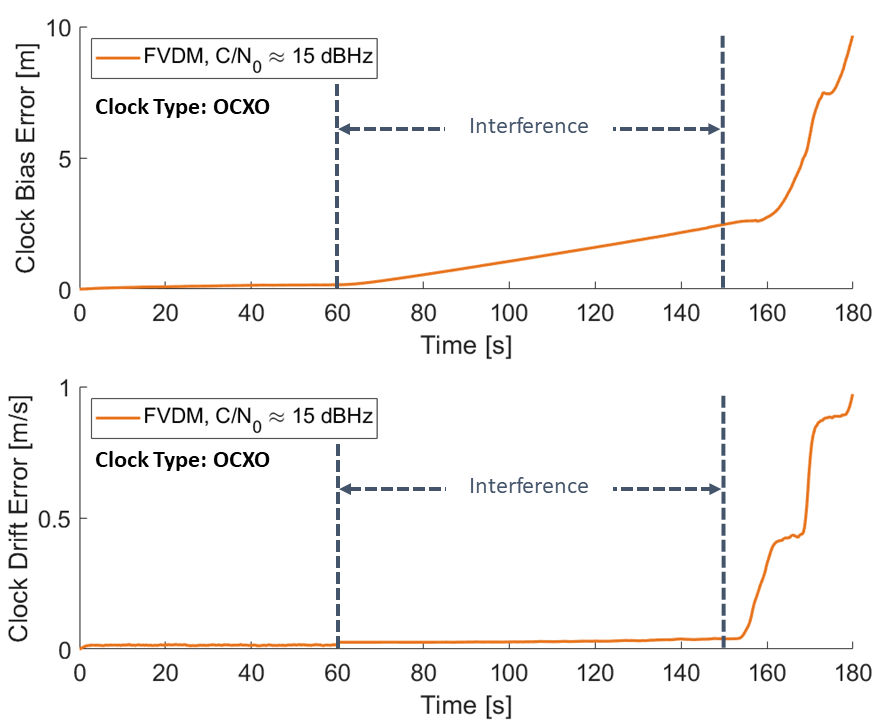
\includegraphics[width=0.75\linewidth]{Figures/Results/trajectoryfigure/Slide20.PNG}
    \caption{Clock bias and Clock drift estimates using the proposed navigation filter when subject to instantaneous interference, bringing the \(C/N_0\) to \(15\) dB-Hz.}\label{fig:Clk15}
\end{figure}

\begin{figure}[!ht]
    \centering
    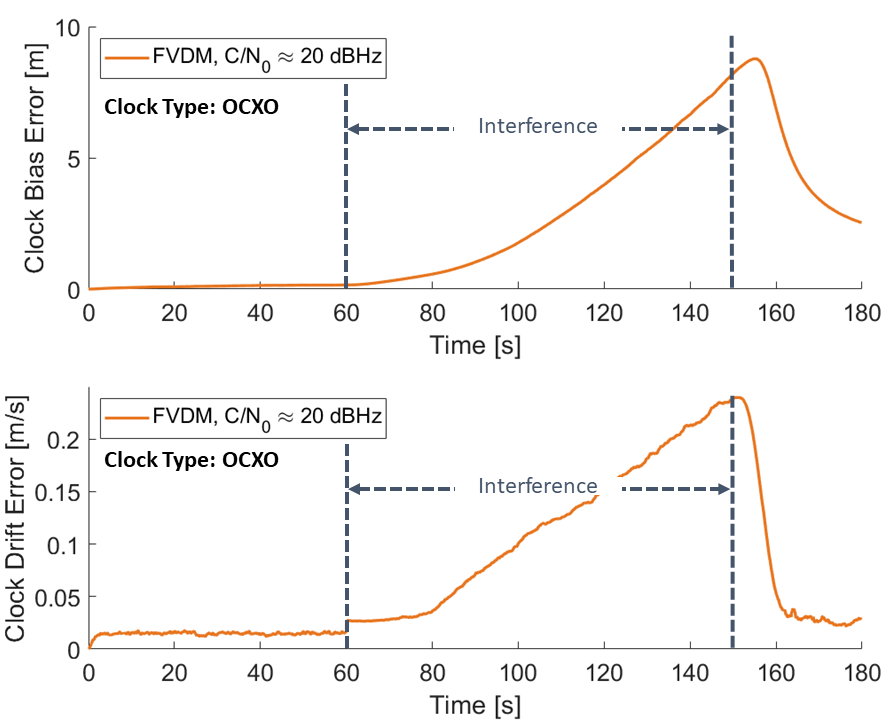
\includegraphics[width=0.75\linewidth]{Figures/Results/trajectoryfigure/Slide21.PNG}
    \caption{Clock bias and Clock drift estimates using the proposed navigation filter when subject to instantaneous interference, bringing the \(C/N_0\) to \(20\) dB-Hz.}\label{fig:Clk20}
\end{figure}

\begin{figure}[!ht]
    \centering
    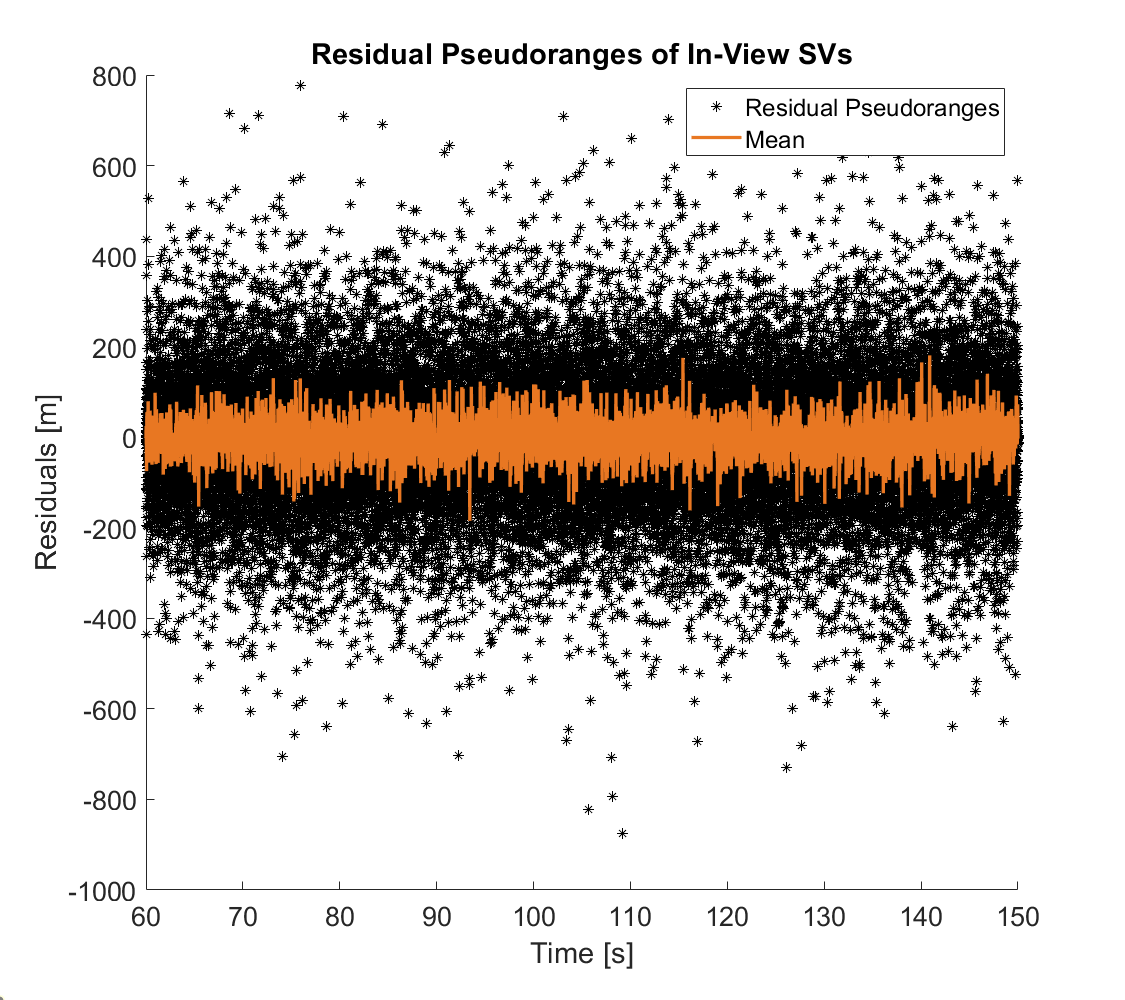
\includegraphics[width=0.75\linewidth]{Figures/Results/Scenario1/Case20/codephase.png}
    \caption{Measurements of code phase in meters from the nine available satellites during interference when \(C/N_0\) is \(20\) dB-Hz.}\label{fig:codephase20}
\end{figure}

\begin{figure}[!ht]
    \centering
    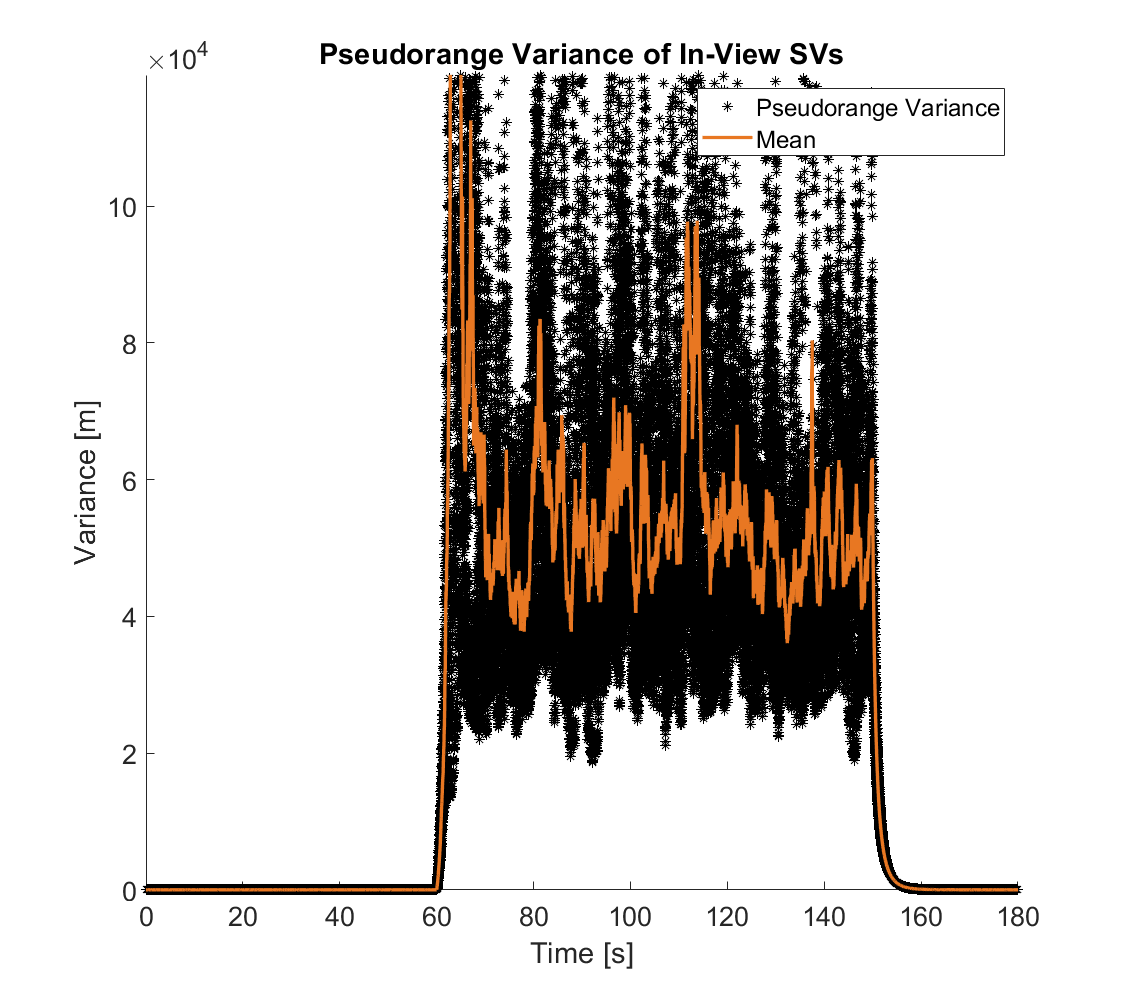
\includegraphics[width=0.75\linewidth]{Figures/Results/Scenario1/Case20/codeVariance.png}
    \caption{Code phase measurement variance in meters from the nine available satellites during interference when \(C/N_0\) is \(20\) dB-Hz.}\label{fig:codephaseVariance20}
\end{figure}

\begin{figure}[!ht]
    \centering
    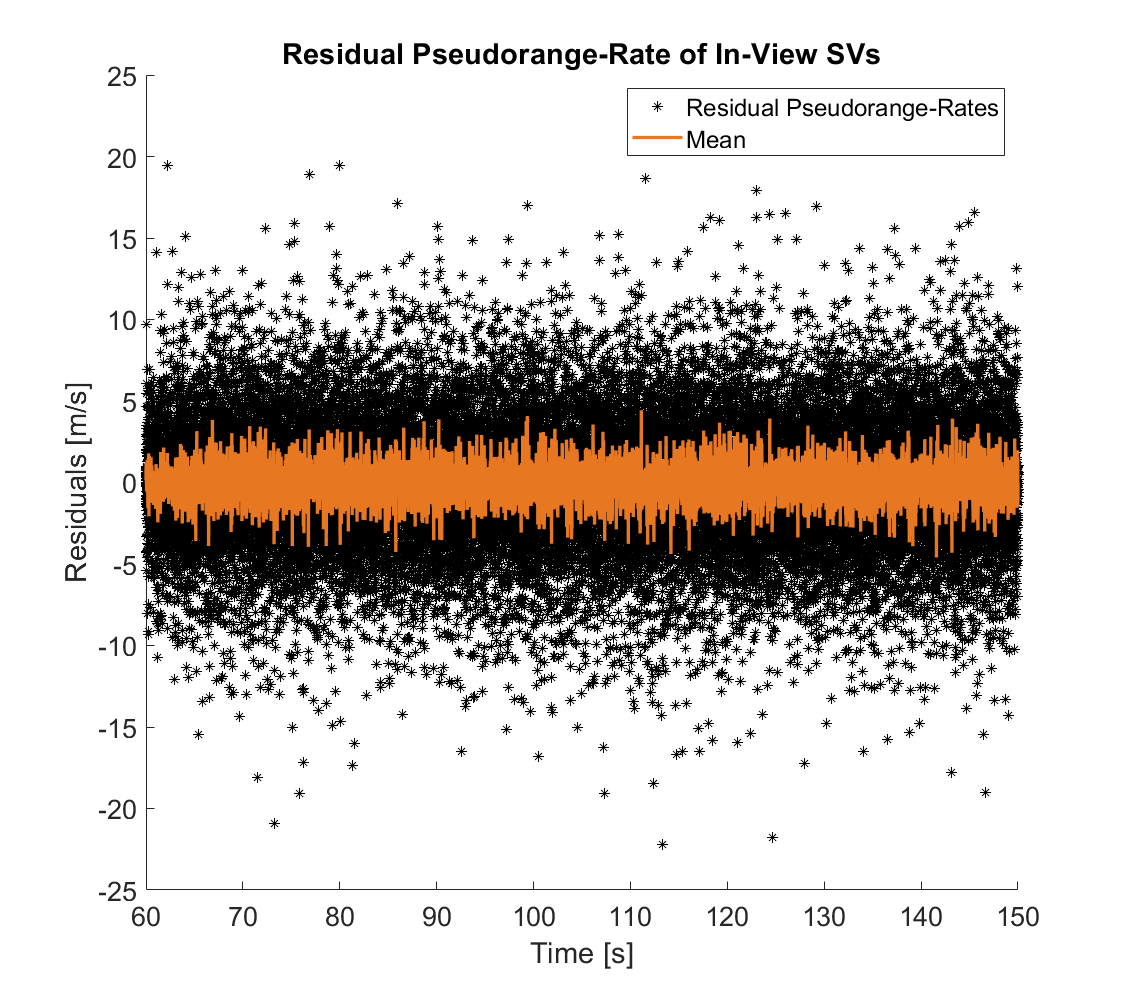
\includegraphics[width=0.75\linewidth]{Figures/Results/Scenario1/Case20/carrierFreq.png}
    \caption{Measurements of carrier frequency in meters per second from the nine available satellites during interference when \(C/N_0\) is \(20\) dB-Hz.}\label{fig:carrier20}
\end{figure}

\begin{figure}[!ht]
    \centering
    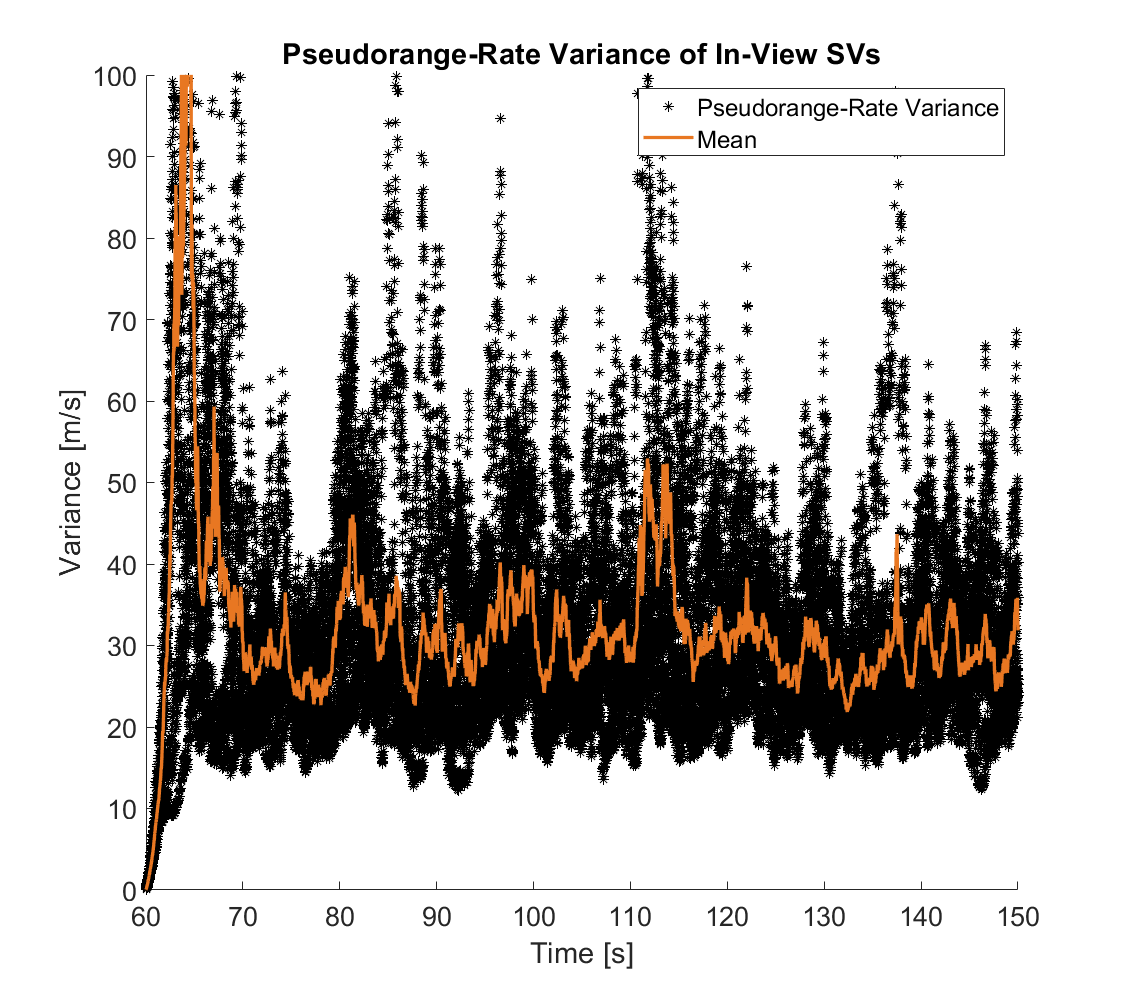
\includegraphics[width=0.75\linewidth]{Figures/Results/Scenario1/Case20/carrierVariance.png}
    \caption{Carrier frequency measurement variance in meters per second from the nine available satellites during interference when \(C/N_0\) is \(20\) dB-Hz.}\label{fig:carrierVariance20}
\end{figure}

\section{\textbf{Scenario 2}}

\subsection{\textbf{Interference Overview}}

\begin{figure}[!ht]
    \centering
    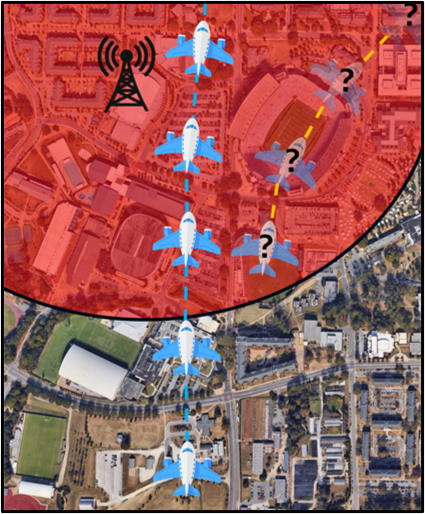
\includegraphics[width=0.75\linewidth]{Figures/notationalinterference.png}
    \caption{Notational image of aircraft flying into interference and accumulating error of its position over time.}\label{fig:notationalinterference}
\end{figure}

\begin{figure}[!ht]
    \centering
    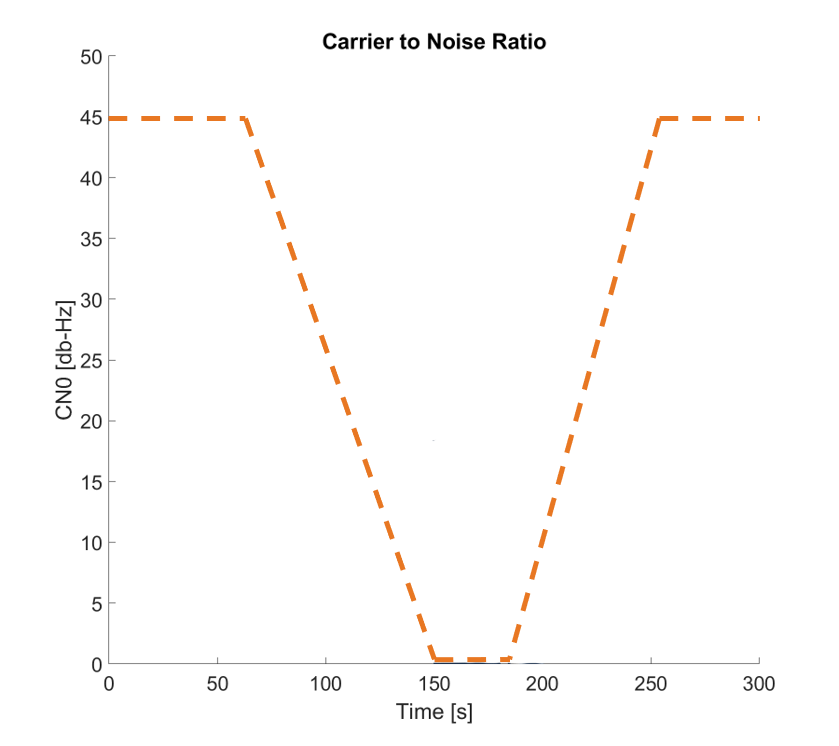
\includegraphics[width=0.75\linewidth]{Figures/Results/CN0scene2.png}
    \caption{Estimated \(C/N_0\) compared with a design \(C/N_0\) that increases interference as aircraft flies closer, and dissipates as aircraft leaves interference zone. }\label{fig:CN0scene2}
\end{figure}

\subsection{\textbf{Monte-Carlo Analyses}}

\begin{figure}[!ht]
    \centering
    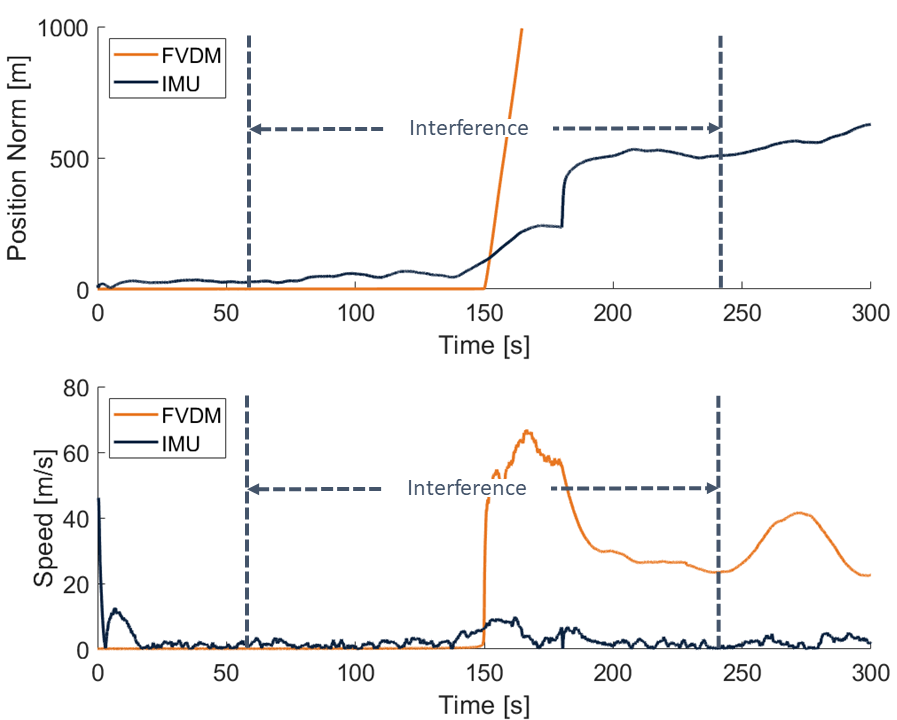
\includegraphics[width=0.75\linewidth]{Figures/Results/trajectoryfigure/Slide19.PNG}
    \caption{Position and speed estimates using the proposed navigation filter when subject to interference that grows stronger as the flight vehicles travels closer to the emitter.}\label{fig:PosVelScene2}
\end{figure}


\begin{figure}[!ht]
    \centering
    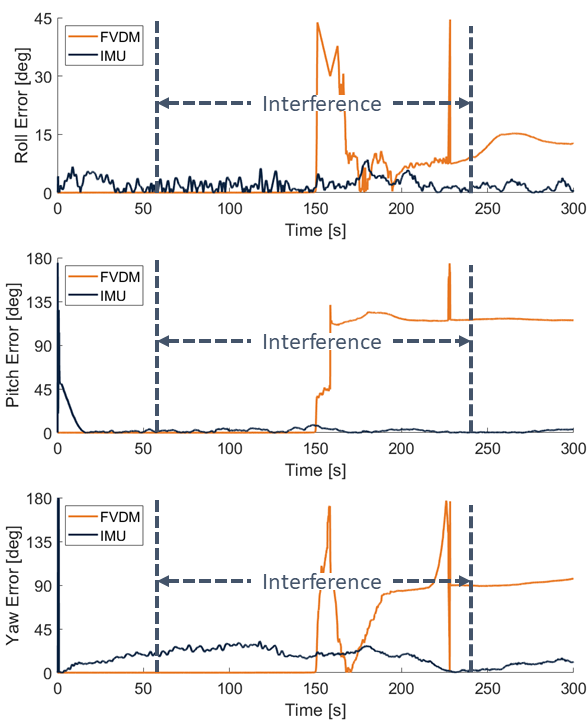
\includegraphics[width=0.75\linewidth]{Figures/Results/trajectoryfigure/Slide7.PNG}
    \caption{Position and speed estimates using the proposed navigation filter when subject to interference that grows stronger as the flight vehicles travels closer to the emitter.}\label{fig:EulScene2}
\end{figure}


\begin{figure}[!ht]
    \centering
    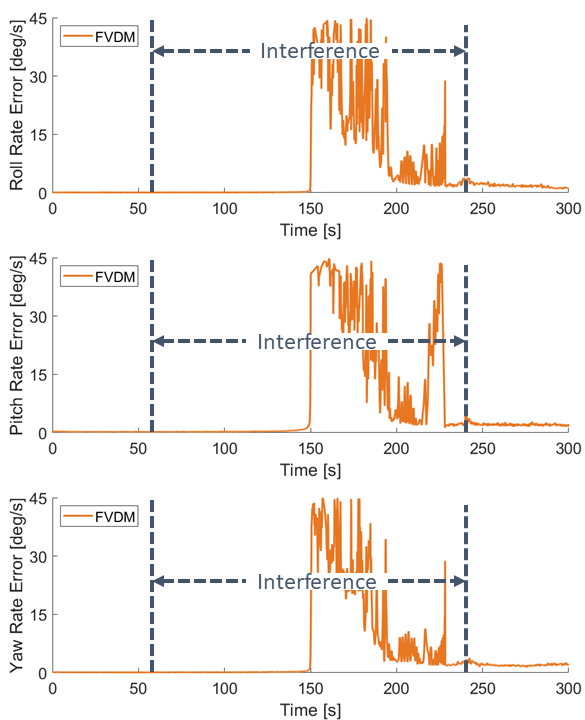
\includegraphics[width=0.75\linewidth]{Figures/Results/trajectoryfigure/Slide13.PNG}
    \caption{Position and speed estimates using the proposed navigation filter when subject to interference that grows stronger as the flight vehicles travels closer to the emitter.}\label{fig:AngScene2}
\end{figure}


\begin{figure}[!ht]
    \centering
    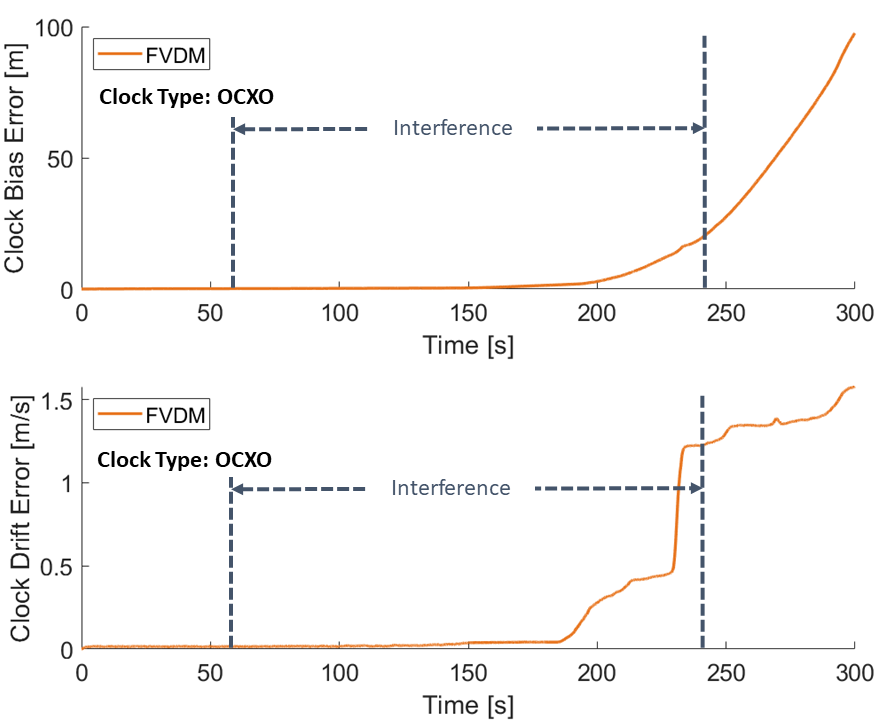
\includegraphics[width=0.75\linewidth]{Figures/Results/trajectoryfigure/Slide25.PNG}
    \caption{Position and speed estimates using the proposed navigation filter when subject to interference that grows stronger as the flight vehicles travels closer to the emitter.}\label{fig:ClkScene2}
\end{figure}


\section{\textbf{Conclusions}}

This chapter presented a detailed explanation of the trajectory used for the Monte-Carlo results in both scenario one and scenario two. The trajectory is a variable-bank, constant-pitch flight path in order to attain estimates of the angular rates and Euler attitude of the aircraft during simulation. Apart of each scenario description was the overview of interference. Scenario one featured sudden drops in signal power to gauge the ability of the vector tracking loops to maintain lock at different levels of signal degradation. Scenario two featured a more realistic interference scenario where the strength of the interference grew as the aircraft flew closer to the emitter location. Based on the results, the FVDM attains better state estimates when the signal interference maintains the \(C/N_0\) about \(15\) dB-Hz. Once the interference was strong enough for the vector tracking loops to drop each channel, the estimates of IMU showed massive improvements over the FVDM {--} this is most-likely due to the constant measurement of angular rate from the gyroscope. The results presented in this chapter show that FVDM is a viable solution to small SWaP-C flight vehicles in benign environments. However, the results also show that the FVDM is not the sole-solution due to the unobservable angular states in GPS-denied conditions. Perhaps external sensors such as a IMU or multi-antenna GPS system could improve the system observability for better estimates. Improvements to the proposed navigation filter are discussed in greater details in the next chapter.